\section{Module 5. Non-stationary noise filtering 2}

Unbiased Non-Local Means algorithm was implemented based on \cite{5a1}. Some, it is believed, improvements to original idea were introduced and described below. Implementation of the UNLM algorithm was divided into several steps:
\begin{itemize}
	\item rewriting NLM prototype from MATLAB to Python,
	\item refactoring to UNLM,
	\item testing different Gaussian kernels,
	\item optimization of algorithm in order to reduce execution time,
	\item adjusting the algorithm to fit both types of data (structural and diffusion weighted).
\end{itemize}
Because some works and further improvements were done in parallel it is hard to describe implementation in chronological order.

\subsection*{Comparison of different Gaussian kernels}
Once the main body of algorithm was ready, it was decided to run some tests to examine the influence of various Gaussian kernels on the output of the UNLM function. The main requirement for the Gaussian kernel was the fact that the overall sum of all elements within kernel should be equal to 1. Another, for sake of sanity, requirement built on the shape of the kernel surface - the slope should be gentle in order to avoid 'overfitting' to the central pixel.

\begin{figure}[H]
\centering{}
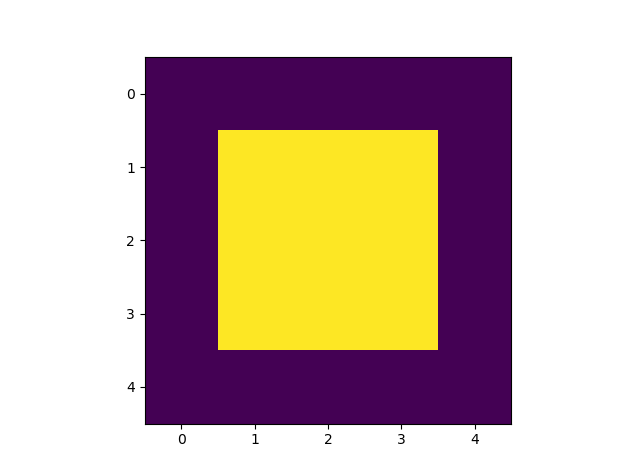
\includegraphics[scale=0.7]{figures/module05/gk1}
\caption{First tested Gaussian kernel.} 
\end{figure}

\begin{figure}[H]
	\centering{}
	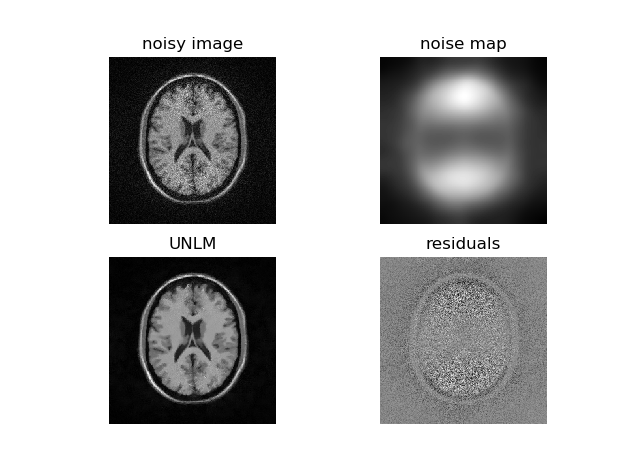
\includegraphics[scale=1]{figures/module05/gk1results}
	\caption{Results obtained for first kernel.} 
\end{figure}

First kernel was presented in the article describing the algorithm \cite{5a1}. However, kernel was considered as not optimal due to its two-level shape. To overcome the problem of wrong shape another attempt took place. Second generated kernel had desired shape, yet values didn't meet the requirement of summing to 1.

\begin{figure}[H]
	\centering{}
	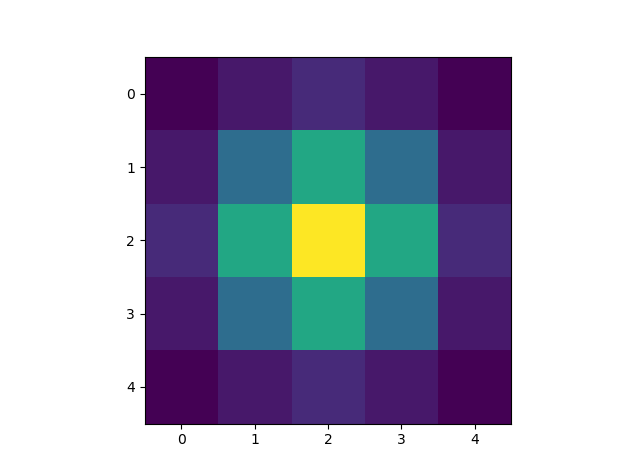
\includegraphics[scale=0.7]{figures/module05/gk2}
	\caption{Second tested Gaussian kernel.} 
\end{figure}

\begin{figure}[H]
	\centering{}
	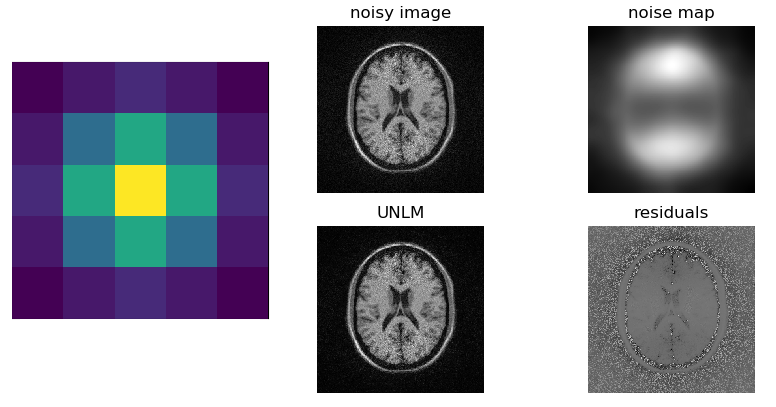
\includegraphics[scale=0.8]{figures/module05/gk2results}
	\caption{Results obtained for second kernel.} 
\end{figure}  

Third kernel, again was disappointing. It had a shape of first kernel, but represented different values, since it was generated in other manner.

\begin{figure}[H]
	\centering{}
	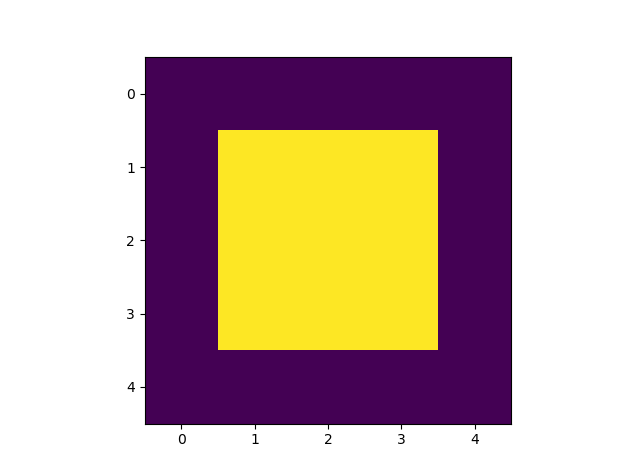
\includegraphics[scale=0.7]{figures/module05/gk3}
	\caption{Third tested Gaussian kernel.} 
\end{figure}

\begin{figure}[H]
	\centering{}
	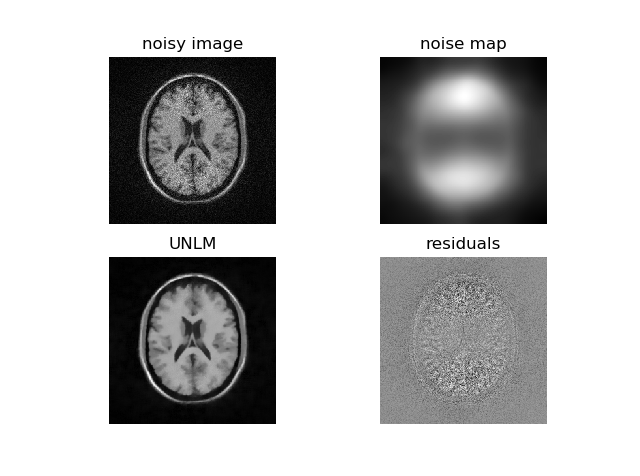
\includegraphics[scale=0.8]{figures/module05/gk3results}
	\caption{Results obtained for third kernel.} 
\end{figure}

Fourth kernel, had all properties that were desired. It was decided to use this particular one in implementation of the UNLM algorithm.

\begin{figure}[H]
	\centering{}
	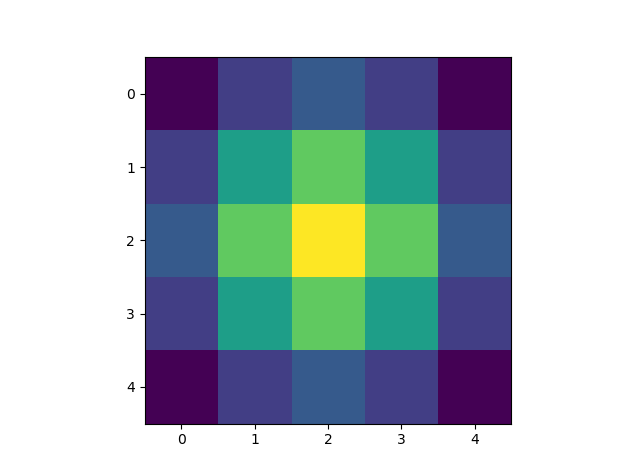
\includegraphics[scale=0.7]{figures/module05/gk4}
	\caption{Fourth, and final, tested Gaussian kernel.} 
\end{figure}

\begin{figure}[H]
	\centering{}
	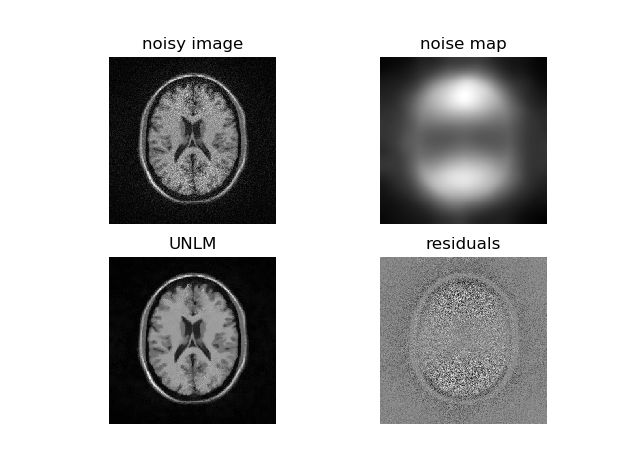
\includegraphics[scale=1]{figures/module05/gk4results}
	\caption{Results obtained for fourth kernel.} 
\end{figure}

Someone with an eye for detail can spot the differences between results achieved whilst using all kernels. Most eye-catching distinction lies in boundaries of the brain and skull.   


Following code snippet presents the implementation of Gaussian window, that was finally chosen after running some tests. This particular window has a special characteristic of being shallow - the central pixel's value doesn't stand out from values in close vicinity. 

\begin{lstlisting}[language=Python, caption = Code used for Gaussian kernel generation.]
def gk4(rsim):

# function that prepares Gaussian window used to penalize
# pixels based on distance within window
kerlen = 2 * rsim + 1
nsig = 2
interval = (2*nsig+1.)/kerlen
x = np.linspace(-nsig-interval/2., nsig+interval/2., kerlen+1)
kern1d = np.diff(st.norm.cdf(x))
kernel_raw = np.sqrt(np.outer(kern1d, kern1d))
kernel = kernel_raw/kernel_raw.sum()
return kernel
\end{lstlisting}

\subsection*{Reducing execution time}
After line-by-line translation of code from MATLAB to Python filtration of single slice lasted for 180 seconds. That was unacceptable, so few flaws in the code had to be identified. It's worth mentioning that single slice filtering in MATLAB took 19 seconds on average.

The first faced incorrectness was the fact of not fully using the numpy library utilities. Changing 'pure python' functions like \textit{sum} to numpy equivalents allowed reduction of time to 80 seconds per slice. That run time was still insufficient. After code profiling with \textit{cProfile} library it was identified, that nested for loops used to move around image were most time consuming. As a result it was decided to get rid off loops and change tedious loop-based architecture to multi-dimensional matrices operations. That operation resulted in achieving 3.5 seconds on average. Involving matrices operations allows to fully exploit numpy implementation (which itself is based on C, so it is faster than Python).

Furthermore, an attempt to use threads in order to speed up calculations on multi-dimensional data took place. For that test, a synthetic 3D data was generated. Processing each slice in a for loop takes 3.5 x \textit{number of slices} seconds. Involving threads should reduce the time, but unfortunately it was doubled. So a tough decision of processing slices in classic loop has been made. Other possibilities of parallel computing were not taken into consideration due to the compatibility issues with GUI.

\subsection*{Unbiased Non-Local Means algorithm}
Having reduced the computation time and having chosen suitable penalty function (Gaussian kernel) algorithm presents as in code snippet below.

\begin{lstlisting}[language=Python, caption = UNLM algorithm code.]
def unlm(image, n_map):

# setting window sizes to reduce number of parameters and chance failure caused by user
rsearch = 5
rsim = 2

# get size for indexes
[m, n] = image.shape

# extend image at boundaries to make calculations on edges of image possible
img_ext = np.pad(image, rsim, 'symmetric')

# create penalty function
penalty = np.asarray(gk4(rsim))

# set space for filtered image
output = np.zeros([m, n])

# precompute possible window2
window2_precomp = np.zeros((m, n, rsearch, rsearch))
for i in range(2, m):
for j in range(2, n):
window2_precomp[i, j, :, :] = img_ext[i - rsim:i + rsim + 1, j - rsim:j + rsim + 1]

# p pixel loop
for i in range(0, m):
for j in range(0, n):
ii = i + rsim
jj = j + rsim
window1 = np.asarray(img_ext[ii - rsim:ii + rsim + 1, jj - rsim:jj + rsim + 1])

# limit the search space
pmin = max(ii - rsearch-1, rsim)
pmax = min(ii + rsearch - 1, m)
qmin = max(jj - rsearch-1, rsim)
qmax = min(jj + rsearch - 1, n)

# define placeholders for values
w_max = 0
avg = 0
w_sum = 0

# set exponential decay
h_sq = 1 / np.square(1.22 * n_map[i, j])

window2_slice = window2_precomp[pmin:pmax, qmin:qmax, :]
window_diff = window1[None, None, :, :] - window2_slice
d = np.sum(penalty[None, None, :, :] * (window_diff * window_diff), axis=(2, 3))

w = np.exp((-1)*d * h_sq)

# primitive way of handling case: pixel p == pixel q
w[w == 1] = -100
w_max = np.amax(w)
w[w == -100] = w_max

w_sum = np.sum(w, axis=(0, 1))
avg = np.sum(w * img_ext[pmin:pmax, qmin:qmax], axis=(0, 1))

avg = avg + w_max * img_ext[ii, jj]
w_sum = w_sum + w_max

if w_sum > 0:
value = avg / w_sum
output[i, j] = abs(cmath.sqrt(value * value - 2 * (np.square(n_map[i, j]))))
else:
output[i, j] = image[i, j]

return output
\end{lstlisting}

To explain the code and present it in more picturesque way, one can look at the image filtering as moving set of
2D windows on image and calculating some metrics, according to their positions and values. There are two types of windows: neighbourhood and search space. Size of neighbourhood window is indirectly defined by rsim parameter, which was assigned by default to 2. That results in neighbourhood window of size 5x5, becasue 5 = 2 * rsim +1. Search space window is dependent ot rsearch parameter, which was assigned to 5 giving 11x11 window. The values of these parameters were set based on analysis conducted in \cite{5a1}. Authors discovered that these sizes give best results in filtration.

Neighbourhood windows are centered around pixels p and q, which are pixel being filtered and filtering pixel correspondingly. Figure below presents the idea of moving windows.

\begin{figure}[H]
	\centering{}
	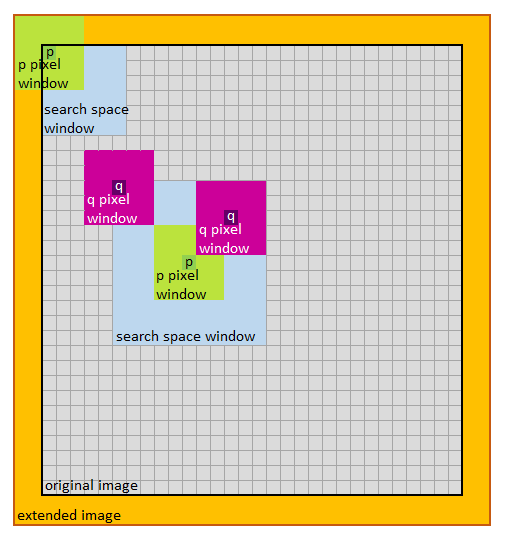
\includegraphics[scale=0.7]{figures/module05/m5windows}
	\caption{Graphical representation of moving windows.} 
\end{figure}

Given figure has to be explained. Gray area represents 2D picture, the grid on in resembles pixels. Dark green square (pixel) is the p pixel and the light green area around it is the neighbourhood window defined by rsim. Similarly, purple area and dark purple pixel resembles window of pixel q. The size of the image has to be extended by rsim in each direction to make calculations on edges of original image possible. This scenario is presented in the top left corner of picture. Pixel p is within area of image but its window doesn't fit into original image. As a consequence of extending the image, the orange area is temporarily added to the image. The values in the added space are assigned by symmetrical padding near edges. Last thing that has to be deciphered is blue square. It is the search space window. It narrows the possibilities of q pixel positions taken into consideration whilst calculating distances between p and q windows.

It is worth mentioning that there exist special case, when q pixel is in the same position as p pixel. If that situation would have been treated equally to other, what would introduce some bias towards 'self-distance'. According to the equation used to calculate distance (d) between windows, one has to calculate element-wise difference of windows. Having both windows in the same position would result in distance equal to 0, which further can have negative influence on the output. To overcome this problem, maximum weight found within the window is assigned to a weight calculated based on 'zero' distance.


\subsection*{Adjusting the algorithm for both types of data}
Denoising using UNLM method is used by both data types, structural and diffusion weighted. There are some differences in implementation of the algorithm for both types, however the same code is used for them in this module. It is caused by analysis of diagrams presented in \cite{5a2}. They showed that taking gradient information gives no significant information in filtering result. On this occasion, the only difference in handling both types of data lays in main function of the module. More precisely, after making decision which data is being processed loops work on different dimensions. Following code snippet presents the \textit{run\_module} function, where data is being accurately handled.

\begin{lstlisting}[language=Python, caption = run\_module function.]
def run_module(mri_input, other_arguments=None):

if isinstance(mri_input, smns.mri_diff):
[m, n, slices, grad] = mri_input.diffusion_data.shape
data_out = np.zeros([m, n, slices, grad])

for i in range(slices):
for j in range(grad):
data_out[:, :, i, j] = unlm(mri_input.diffusion_data[:, :, i, j], mri_input.noise_map[:, :, i, j])

mri_input.diffusion_data = data_out

elif isinstance(mri_input, smns.mri_struct):
[m, n, slices] = mri_input.structural_data.shape
data_out = np.zeros([m, n, slices])

for i in range(slices):
data_out[:, :, i] = unlm(mri_input.structural_data[:, :, i], mri_input.noise_map[:, :, i])

mri_input.structural_data = data_out

else:
return "Unexpected data format in module number 5!"

return mri_input
\end{lstlisting}

One decision must be finally justified. The whole bigger product is targeted (theoretically) at physicians that usually have no knowledge of image filtering. On this occasion it was decided to reduce number of parameters responsible for algorithm outcome to 0. That solution should reduce possibilities of getting badly-processed data, as optimal parameters are set by default.
